\documentclass[12pt]{article}
\usepackage[margin=1.5cm]{geometry}
\usepackage{parskip}
\usepackage{amsmath}
\usepackage{amssymb}
\usepackage{amsfonts}
\usepackage{enumitem}
\usepackage{graphicx}
\usepackage{stmaryrd}
\graphicspath{ {./images/} }


\begin{document}
\begin{enumerate}[label=(\alph*)]

  \item
    Not relevant.

  \item

    For finding global alignment between two DNA sequences, we use the Needleman-Wunsch algorithm.

    This is a dynamic programming algorithm for sequences $x$ and $y$.

    It involves creating a $|x| \times |y|$ matrix, where the cell $(i,j)$ represents the similarity score for the best alignment between subsequences $x_1\ldots x_i$ and $y_1\ldots y_j$, so the alignment score for the entires sequence is found in the bottom-right cell.

    We initialise by filling in cells $F(0,i) = -i \cdot d$ and $F(j,0)$ with $-j \cdot d$, for all $i$ and $j$, where $d$ is the gap penalty.

    Then, to fill in the remainder of cells, we use the following equation:

    $F(i,j) = \max\begin{cases}F(i -1, j) - d\\F(i, j-1) - d\\F(i-1, j-1) + s(x_i, y_j)\end{cases}$

    Where $s(x_i, y_j)$ give us the match/mismatch score between two characters.

    The first two cases correspond to putting a gap in the first or second sequence, and the final case corresponds to a match/mismatch.

    To obtain an alignment, we generate an auxiliary $Ptr$ matrix, which we fill in with the direction to go to backtrack, based on which case we chose for the calculation of the corresponding $F(i,j)$.

    We present an example, finding an alignment between sequences, using the given parameters:

\begin{verbatim}
AGGCAT
AGCCCT
\end{verbatim}

We get:

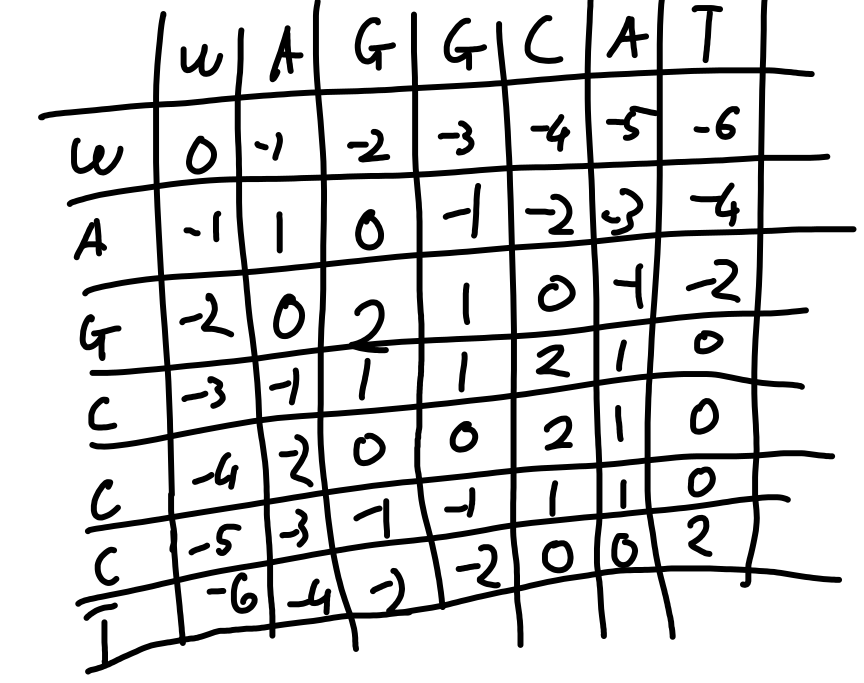
\includegraphics[scale=0.3]{alignment}

And therefore we obtain the following alignment:

\begin{verbatim}
AGGCAT
AGCCCT
\end{verbatim}



  \item
    Not relevant.

        
    \end{enumerate}
\end{document}
